\documentclass[12pt, aspectratio=169]{beamer}
\usepackage{
    hyperref,
    graphicx,
    % enumitem,
    transparent,
    siunitx,
    pgfpages,
    caption,
    booktabs,
    multirow,
    bm,
    standalone,
    tikz,
    comment,
    xcolor,
    svg,
}
\usepackage[hang,flushmargin]{footmisc}
\setbeameroption{hide notes}
% \setbeameroption{show only notes}
% \setbeameroption{show notes on second screen}
\setbeamertemplate{note page}[plain]
\setbeamercovered{transparent}

% get rid of junk
\usetheme{default}
\usecolortheme{orchid}
\beamertemplatenavigationsymbolsempty
\hypersetup{pdfpagemode=UseNone} % don't show bookmarks on initial view

% named colors
\definecolor{offwhite}{RGB}{249,242,215}
\definecolor{foreground}{RGB}{255,255,255}
\definecolor{background}{RGB}{24,24,24}
\definecolor{title}{RGB}{107,174,214}
\definecolor{gray}{RGB}{155,155,155}
\definecolor{subtitle}{RGB}{102,255,204}
\definecolor{hilight}{RGB}{102,255,204}
\definecolor{vhilight}{RGB}{255,111,207}
\definecolor{lolight}{RGB}{155,155,155}
%\definecolor{green}{RGB}{125,250,125}

% use those colors
\setbeamercolor{titlelike}{fg=title}
\setbeamercolor{subtitle}{fg=subtitle}
\setbeamercolor{institute}{fg=gray}
\setbeamercolor{normal text}{fg=foreground,bg=background}
\setbeamercolor{item}{fg=foreground} % color of bullets
\setbeamercolor{subitem}{fg=foreground}
\setbeamercolor{itemize/enumerate subbody}{fg=foreground}
\setbeamercolor{section in toc}{fg=title}
\setbeamercolor{alerted text}{fg=title}

\setbeamertemplate{itemize subitem}{{\textendash}}
\setbeamerfont{itemize/enumerate subbody}{size=\footnotesize}
\setbeamerfont{itemize/enumerate subitem}{size=\footnotesize}

\addtobeamertemplate{block alerted begin}{%
  \setbeamercolor{alerted text}{fg=red}%
}{}
\addtobeamertemplate{block example begin}{%
  \setbeamercolor{alerted text}{fg=green}%
}{}

% add a bit of space at the top of the notes page
\addtobeamertemplate{note page}{\setlength{\parskip}{12pt}}

% a few macros
\setbeamertemplate{description item}{
    \hfill\alert{\textbf{\insertdescriptionitem}}
}
\setbeamertemplate{itemize items}[circle]

\AtBeginSection[]{
    \begin{frame}
        \vfill
        \centering
        \Huge\color{title}\insertsectionhead
        \vfill
    \end{frame}
}

\newcommand\blfootnote[1]{%
    \begingroup
    \renewcommand\thefootnote{}\footnote{\tiny \color{lolight} #1}%
    \huge%
    \addtocounter{footnote}{-1}%
    \endgroup
}

% math macros
\renewcommand{\d}[1]{\mathsf{d}#1}
\newcommand{\diff}[2]{\frac{\mathsf{d} #1}{\mathsf{d} #2}}
\newcommand{\ddiff}[2]{\frac{\mathsf{d}^2 #1}{\mathsf{d} {#2}^2}}
\newcommand{\pdiff}[2]{\frac{\partial #1}{\partial #2}}
\renewcommand\vec{\bm}
\newcommand{\uvec}[1]{\vec{\hat{#1}}}
\newcommand{\grad}{\vec{\nabla}}
\newcommand{\prandtl}{\ensuremath{\mathsf{Pr}}}
\newcommand{\rayleigh}{\ensuremath{\mathsf{Ra}}}
\newcommand{\nusselt}{\ensuremath{\mathsf{Nu}}}

% text macros
\newcommand{\rb}{Rayleigh-B\'{e}nard}

\title{
    Data-driven subgrid-scale parametrisation for a simple dynamical system
}
\subtitle{Honours project update}
\author{Thomas Schanzer}
\institute{
    School of Physics\\
    Climate Change Research Centre and
    ARC Centre of Excellence for Climate Extremes \\
    \vspace{6pt}
    University of New South Wales, Sydney, Australia
}
\date{Thursday 20 July 2023}


\begin{document}

\begin{frame}
\maketitle
\end{frame}

% The aim and motivation
\begin{frame}
The complexity of atmospheric models makes parametrisation testing difficult.
{\center \color{hilight} I aim to:}
\begin{enumerate}
    \item Use a simpler dynamical system as a test-bed
    \item Build data-driven parametrisation schemes from scratch,
        with/without
    \begin{enumerate}[i]
        \item Stochasticity
        \item Memory
    \end{enumerate}
    \item Evaluate the schemes' performance
\end{enumerate}
\end{frame}

% The equations (with hyperdiffusion)
\begin{frame}{\rb{} convection in 2D}
\begin{align*}
    \pdiff{\vec{u}}{t} + \vec{u} \cdot \grad \vec{u}
        &= -\grad \pi + \left( \frac{\prandtl}{\rayleigh}\right)^{1/2}
        \left( 1 + {\color{hilight} \nu^* |\nabla^2 \vec{u}|} \right)
        \nabla^2 \vec{u} + \theta \uvec{z} \\
    \pdiff{\theta}{t} + \vec{u} \cdot \grad \theta
        &= (\rayleigh\,\prandtl)^{-1/2}
        \left( 1 + {\color{hilight} \nu^* |\nabla^2 \theta|} \right)
        \nabla^2 \theta \\
    \grad \cdot \vec{u} &= 0
\end{align*}
\begin{itemize}
    \item Rayleigh number $\rayleigh = 10^9$ $\Rightarrow$ turbulent
    \item Prandtl number $\prandtl = 1$
    \item {\color{hilight} Nonlinear hyperdiffusion} for model stability at low
        resolution ($\nu^* = 10^{-3}$)
    \item No-slip, isothermal top/bottom boundaries; periodic lateral boundaries
\end{itemize}
\end{frame}

% Numerical methods
\begin{frame}{Numerical methods}
\begin{itemize}
    \item Equations solved using \texttt{dedalus} v3: spectral PDE solver
        for Python
    \begin{itemize}
        \item Highly flexible
        \item Designed to run in parallel
    \end{itemize}
    \item Horizontal Fourier series expansion
    \item Vertical Chebyshev polynomial expansion
\end{itemize}
\end{frame}

% Animation
\begin{frame}{Animation}
Integration for 100 time units with 1024 horizontal and 128 vertical modes:
\begin{center}
    \url{https://youtu.be/SU8ColUYYlA}
\end{center}

Key properties:
\begin{itemize}
    \item Turbulent flow
    \item Large and small scale features
    \item Only two prognostic variables
    \item Comparatively inexpensive (13 cpu-hr for the above run)
\end{itemize}

\vspace{3mm}
{\color{hilight} $\Rightarrow$ A simple dynamical system analogue of the
atmosphere}
\end{frame}

\begin{frame}{I need:}
\begin{enumerate}
    \item A reasonably accurate high-resolution model to treat as ``truth''
    \item A coarse-resolution model to correct using parametrisation
    \item Evidence that under-resolution introduces biases that are:
    \begin{enumerate}[i]
        \item \emph{Systematic:} consistent over- or under-estimation,
            not mere numerical error
        \item \emph{Statistically significant}
    \end{enumerate}
\end{enumerate}
\end{frame}

% Define quantities of interest
\begin{frame}{Quantities of interest}
Nusselt number (dimensionless rate of vertical heat transport):
\begin{equation*}
    \nusselt(z,t) \equiv (\rayleigh\,\prandtl)^{1/2} \langle w \theta \rangle_x
        - \pdiff{\langle \theta \rangle_x}{z}
\end{equation*}

Root-mean-square velocity:
\begin{equation*}
    u_\mathsf{rms}(t) = \sqrt{\langle \vec{u} \cdot \vec{u} \rangle_{x,z}}
\end{equation*}

Mean values are obtained via:
\begin{enumerate}
    \item 1000 time unit spin-up at coarse resolution
    \item 300-time-unit integration at new resolution
    \item Averaging over final 275 time units
\end{enumerate}
\end{frame}

% Resolution dependence plots
\begin{frame}{Mean Nusselt number}
\begin{figure}
    \centering
    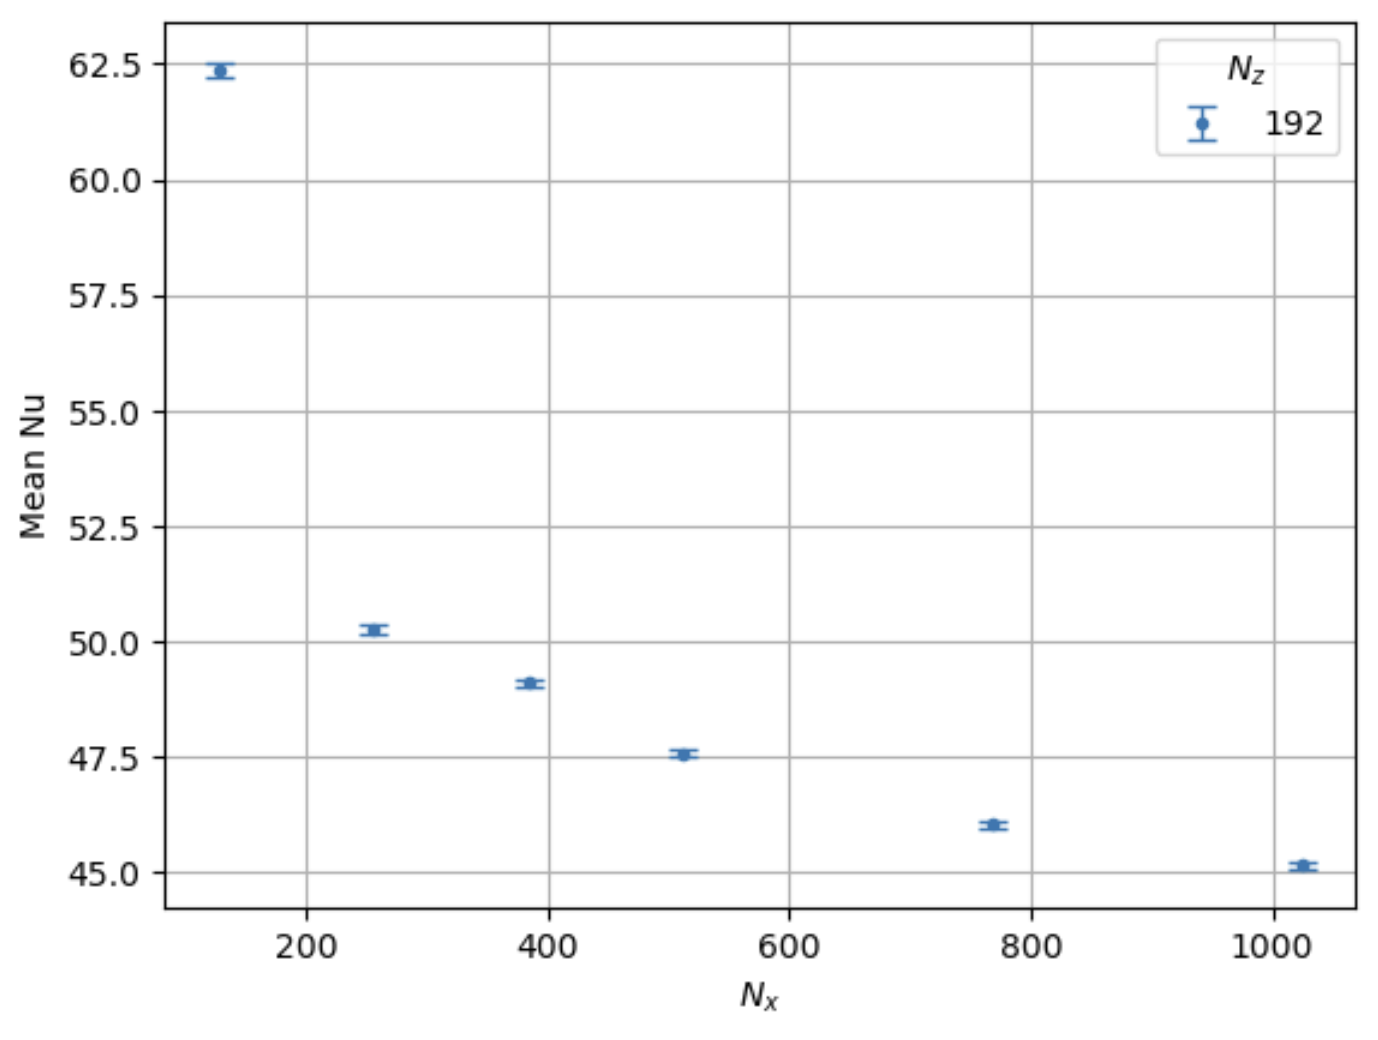
\includegraphics[width=0.6\linewidth]{figures/nu_dependence.png}
\end{figure}
\end{frame}

\begin{frame}{Mean RMS velocity}
    \begin{figure}
        \centering
        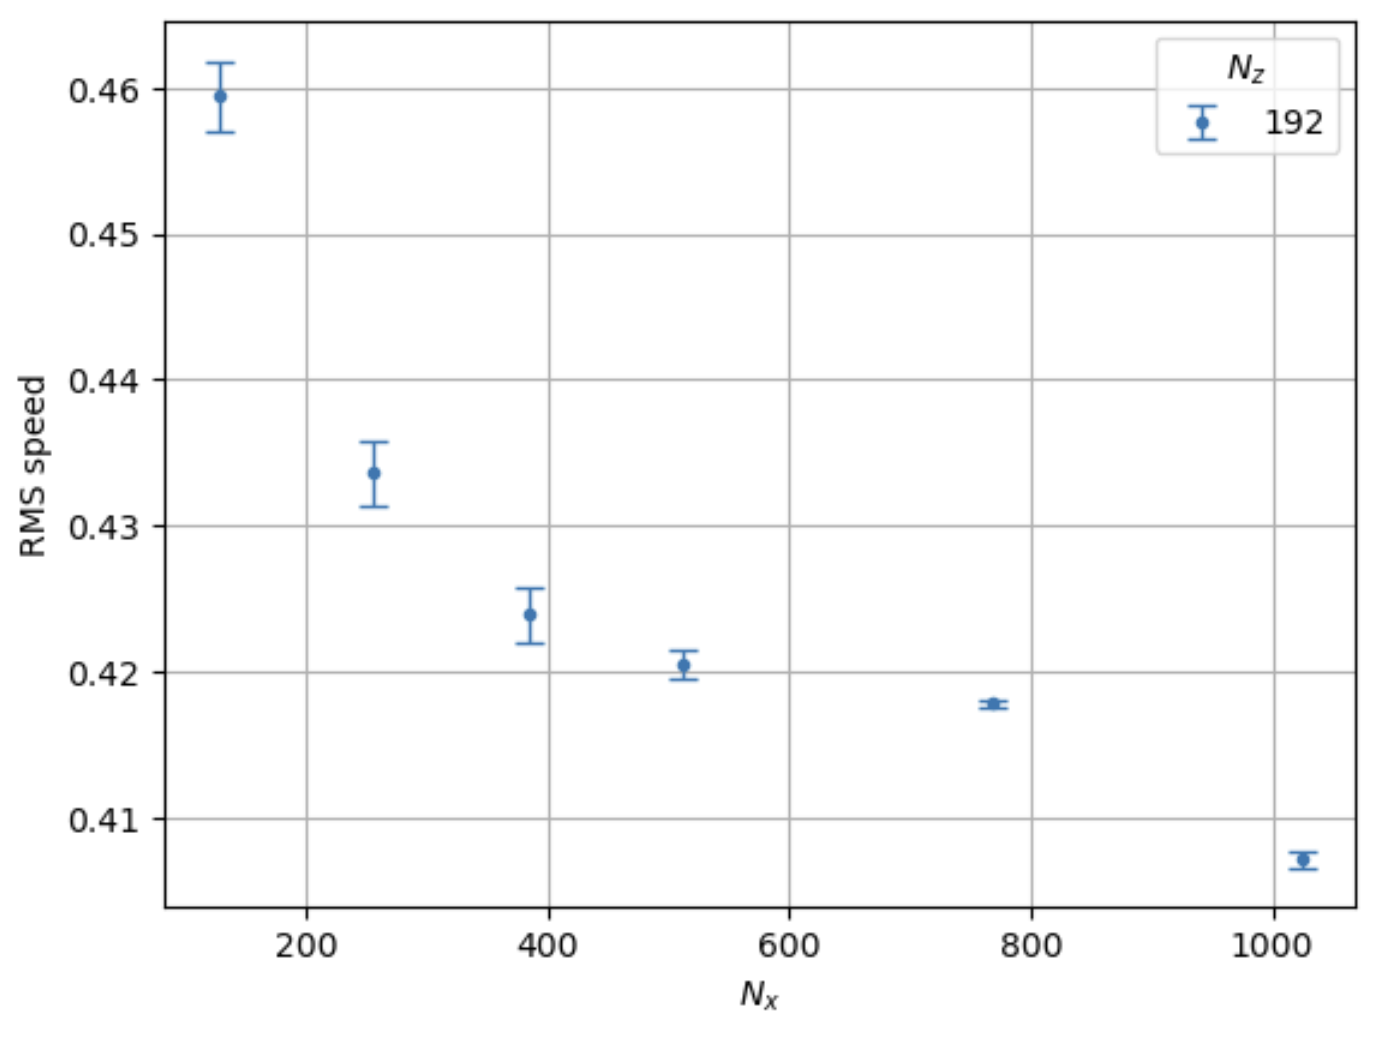
\includegraphics[width=0.6\linewidth]{figures/urms_dependence.png}
    \end{figure}
\end{frame}

% Next steps
\begin{frame}{Next steps: building the parametrisation}
\begin{enumerate}
    \item Given the state $S_t$ of the fine model at time $t$,
    \begin{enumerate}[i]
        \item Advance it by $\Delta t$ using the fine model
            $\mathcal{F}_{\Delta t}$, giving $\mathcal{F}_{\Delta t} S_t$
        \item Coarse-grain it and advance it by $\Delta t$ using the coarse
        model $\mathcal{C}_{\Delta t}$, giving
        $\mathcal{C}_{\Delta t} \langle S_t \rangle$
    \end{enumerate}
    \item Determinine the \emph{unresolved tendency}
        \[
            T = \frac{
                \langle \mathcal{F}_{\Delta t} S_t \rangle
                - \mathcal{C}_{\Delta t} \langle S_t \rangle
            }{
                \Delta t
            }
        \]
    \item Fit a model to the dataset of $(\langle S_t \rangle, T)$
    \item Plug this into the coarse model as an external forcing and
        assess the results
\end{enumerate}
\end{frame}

\end{document}
